boundad problem = time window
data is stationary if statistical attributes like mean SD not vary over the time
non-stationary --> drift

k-means 
which relies on the idea that the center of the cluster, called centroid, can be a good representation of the cluster. The algorithm starts by selecting k cluster centroids. Then the cosine distance2 between each document in the collection and  
centroids is calculated and the document is assigned to the cluster with the
nearest centroid. After all documents have been assigned to clusters, the new cluster centroids are recalculated and the procedure runs iteratively until some
criterion is met. Many variations of the k-means algorithm are proposed, e.g. ISODATA (Jain et al., 1999) and bisecting k-means (Steinbach et al., 2000). 

k-mean algorithm (Kaufman and Rousseauw, 1990)

The K-medoids method is more robust than the K-means algorithm in the
presence of noise and outliers because a medoid is less influenced by outliers
or other extreme values than a mean. However, its processing is more costly
than the K-means method. Both methods require the user to specify K, the
number of clusters.
Other error criteria can be used instead of the SSE. Estivill-Castro (2000)
analyzed the total absolute error criterion. Namely, instead of summing up
the squared error, he suggests to summing up the absolute error. While this
criterion is superior in regard to robustness, it requires more computational
effort.

The K-means algorithm has the following main advantages [100]:
– it is very easy to implement, and
– its time complexity is O(Np) making it suitable for very large data sets.
However, the K-means algorithm has the following drawbacks [25]:
– the algorithm is data-dependent,
– it is a greedy algorithm that depends on the initial conditions, which may cause the algorithm to
converge to suboptimal solutions, and
– the user needs to specify the number of clusters in advance.

Although K-means has the great advantage of being easy to implement,
it has two big drawbacks. First, it can be really slow since in each step the
distance between each point to each cluster has to be calculated, which can
be really expensive in the presence of a large dataset. Second, this method
is really sensitive to the provided initial clusters, however, in recent years ,
this problem has been addressed with some degree of success [23].


K-Means has a few problems however. The first is that it isn’t a clustering algorithm, it is a partitioning algorithm. That is to say K-means doesn’t ‘find clusters’ it partitions your dataset into as many (assumed to be globular) chunks as you ask for by attempting to minimize intra-partition distances. That leads to the second problem: you need to specify exactly how many clusters you expect. If you know a lot about your data then that is something you might expect to know. If, on the other hand, you are simply exploring a new dataset then ‘number of clusters’ is a hard parameter to have any good intuition for. The usually proposed solution is to run K-Means for many different ‘number of clusters’ values and score each clustering with some ‘cluster goodness’ measure (usually a variation on intra-cluster vs inter-cluster distances) and attempt to find an ‘elbow’. If you’ve ever done this in practice you know that finding said elbow is usually not so easy, nor does it necessarily correlate as well with the actual ‘natural’ number of clusters as you might like. Finally K-Means is also dependent upon initialization; give it multiple different random starts and you can get multiple different clusterings. This does not engender much confidence in any individual clustering that may result.


However, the number of
clusters can be controlled by the preference parameter. That is, a high value
of the preference will cause AP to form many clusters, while a low value will
lead to a small number of clusters. If the preference value is not provided
the median similarity or the minimum similarity will be used.



% \section{Summery}

% \begin{table}[ht]
%     \centering
%     \caption{comparison between DSAP version 1 and DSAP version 2 }
%     \label{dsap12}
%     \begin{tabular}{|c|c|c|}
%     \hline
%       & DSAP v.1 & DSAP v.2 \\
%      \hline
%      exemplar &  generate  & actual point\\
%      \hline
%      phases & 2 phase  & 2 phase\\
%      \hline
%       concept drift & no  & yes\\
%      \hline
%     performance &  stable & stable\\
%     \hline
%     handling evolving &  no & yes\\
%     \hline
%     Algorithm based &  AP & AP\\
%     \hline
%     Time Window &  landmark & sliding\\
%      \hline

%     \end{tabular}
    
% \end{table}

% The K-means stream algorithm performed in this work is based on data stream mining framework\cite{hahsler2017introduction} consists of two main components:
% \begin{itemize}
%     \item Data Stream Data or DSD: This stage simulates or connects to the stream of data.
%     \item Data Stream Task or DST: it applies data stream mining task. In this work, we only applies Data Stream Clustering (DSC) task.
% \end{itemize}

%After choosing DSD for stream simulation, the next phase would be to determine a Data Stream Task or DST. DST  assigns to any data mining task that can be utilized to a data stream. Figure \ref{DSR} shows the DST hierarchy with the DSO (Data Stream Operator), DSC (Data Stream Clustering), DSFPM (or Frequent Pattern Mining) sub-classes. In this work, we only focused on data stream clustering or DSC. In DSC, there are different clustering methods, and among them, DSC\_TwoStage is applied to our data.

%To define a full data stream clustering process with an online micro and offline macro phases, \textit{Two\_Stage} framework is applied. This phases are:
%To define a full data stream clustering process with an online and offline algorithm, stream implements a DSC package called DSC\_TwoStage, which can combine DSC\_Micro and DSC\_Macro K-means into a two-stage process. We will go through these two stages below. 

% \begin{figure}
% \centering
% 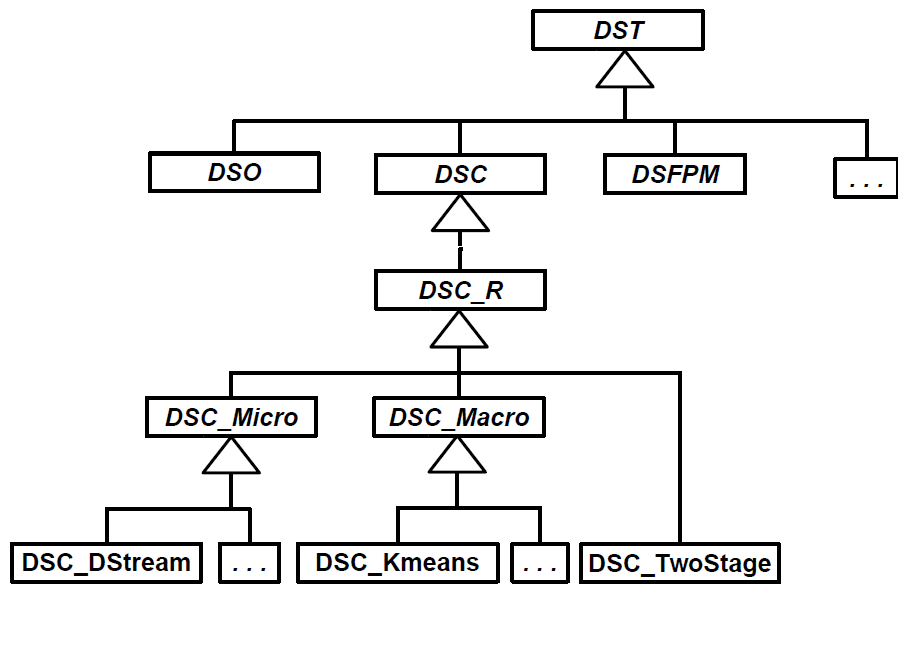
\includegraphics[width = 14cm,height = 9cm]{image/dst.png}
% \caption{Overview of the data stream Data (DSD) class structure}
% \label{DSR}
% \end{figure}

% Next, special class of DSC called DSC\_TwoStage will apply. The micro clustering algorithm used in the online stage or DSC\_micro. There are few function applied in this phase as follow.

% \begin{itemize}
%     \item DSC\_Window provides a clustering interface to the data stream operator DSO\_Window. It implements the sliding window model, which keeps a specified number of the most recent data points of the stream defines by the user. This number is the window length. 
    
%     \item DSC\_Kmeans interface is the R version of K-means clustering implementation and a version of k-means where the data points (micro-clusters) are weighted by the micro cluster weights.
    
%     \item The streaming k-means clustering algorithm requires continuously update the calculation of micro clusters.
    
%     Update function is defined as: update(dsc, dsd, n = 1, verbose = FALSE, ...) which accepts a DSC object and a DSD object. It requests the n data points from dsd and adds them to the clustering
%     in dsc.
    
% \end{itemize}


% \subsection{Data collection }
% Data collection is the process of gathering and measuring information. The data collection method consists of two categories, quantitative and qualitative.
% Experimental research is a quantitative method. Interviews are qualitative methods.
% Surveys, observations, archival research and secondary data collection can be quantitative or qualitative methods.

% In our case study, we have chosen two datasets, people counter from Flinders university and UjiIndoorLoc, an indoor localization dataset.
% People counting dataset is a collection of indoor data based on three months of experiment on the sedentary lifestyle. 
% UjiIndoorLoc dataset is focused on WLAN fingerprint positioning technologies and methodologies (also know as WiFi Fingerprinting).

% Hence, collecting streaming data needs time and facilities, we used two ready to use dataset and apply a stream simulation phase to use as data stream for our model.


% \subsection{Data Preprocessing}
% Data preprocessing is a method that includes transforming raw data into an expected format. Real-world data can be incomplete, inconsistent or having many errors.
% Four data pre-processing steps are applied to deal with the problems may affect our results. They are:

% \begin{itemize}
% \item Data cleaning
% \item Outlier Detection
% \item Data Transformation
% \end{itemize}

    
    %  Threshold $\epsilon$ is computed online according to the rate of change observed from the data point and clusters. It is a heuristic method to adjusts the mean values of the data points and keeps those below a threshold level.
    %  To find the adaptive threshold, first, the data point $x_i$ should find it own cluster with the centroid $C_{mi}$ that consists of $N_i$ number of data points assigned to this cluster. Then, the maximum distance of the centroid $C_{mi}$ from the cluster members $N_i$ is calculated for each cluster and this value is the adaptive threshold.
    %  It important to know that the data point $x_i$ belongs to which cluster. As shown in Figure \ref{thr}, some clusters are dense and some other are spread,  then this number is different for different type of clusters. If we had a fix value for $\epsilon$, If we use T' as a threshold, most of the data points in (a) clusters become outliers.